% !TEX root = /Users/zhuzhuangdi/Desktop/MSUCourses/MachineLearning847/17spr_wang_zhu_du/Final/final_report.tex
\subsection{Data Collection}   
For our experiment, we obtained dataset for both Tang Shi and Song Ci. Many research projects were conducted for automatically generating Tang Shi. So we can evaluate our experiment result by comparing with these machine-created Tang poem. And then we can move forward to Song Ci.

\begin{itemize}
\item \textbf{Tang Poetry Corpus.} We use Quan Tangshi as our Tang Poetry corpus.\cite{1960quantangshi}. It was commissioned by Yin Cao in 1705 and published under the name of Kangxi Emperor. It contains 49,000 lyric poems (in the dataset we used it has 49,274 poems) and is believed the largest collection of Tang poetry. We obtained the dataset from the server of \cite{zhang2014chinese}. The dataset is well organized and is ready to use as the input of our experiments.

\item \textbf{Song Ci Corpus.} We download the Quan Song Ci dataset as our corpus for Song Ci. Quan Song Ci collected 21,116 Song Ci poems (Data set we used contains 18986 poems). Although there are several previous projects, unlike the parsed Tang Poetry Corpus, the dataset we can get is not well-formatted. For our analysis, preprocessing is conducted in the following steps: First, we extracted the name of all poets from the list in collections. Second, then we can distinguish those lines of names and those lines of poems. Third, we filtered the length of text smaller that certain number and without any period in it. Most titles are just the Cipai, some may contain a subtopic. We treat Cipai separately as it set the format of the poem. Fourth, we then identify the title of poems with its main text. Finally, we generate a tab separated file for further process.

\item \textbf {Hybrid Corpus.} Since the number of preserved Song Ci for each Ci Pai is very limited, which makes it difficult to train any neural network, for each Ci Pai, we generate around 1000 Song Ci with the specified Ci Pai using the Genetic Algorithm, and inject them into our dataset for further training the RNN model and GAN model.
\end{itemize}

%
\subsection {Ci Pai Analysis}
%
%The dataset we use contains 18668 Ci, which contains a total number of 1183 poets and 1170 Pai. This dataset basically covers Ci generated during the entire Song Dynasty and the beginning of Yuan Dynasty. 
%We analyze the number of poems wrote by each poet, which shown in Figure \ref{fig:poet}. Most of the poems are created by the first poets. The one that creates the most poems is Qiji Xin, one of the most famous poet of the Southern Song Dynasty. His poems covers a wide range of styles. Among all those poems, the bold style is most will known by now. 
%
We analyze the statistics for different Ci Pai in our corpus. 
%Ci was first used as a lyric, and Pai is the name of the tune. Each Pai has a specific melody and rhythm, so Ci has a fixed format requirements, such as the number of sentences, the number of words per sentence, pronunciation of those words, rhyme and so on. 
%
As shown shown in Figure \ref{fig:Pai}, the most popular Pai is Silk-Washing Stream, followed by Prelude To Water Melody, Partridge Sky, Pusaman and River of Red. 
%And there is good reason to believe that the songs that corresponding to these Pai are beautiful in melody, lively in rhythm and easy to sung, which caused them to be so popular in ancient China.
%\begin{figure}[htbp]
%	\centering
%	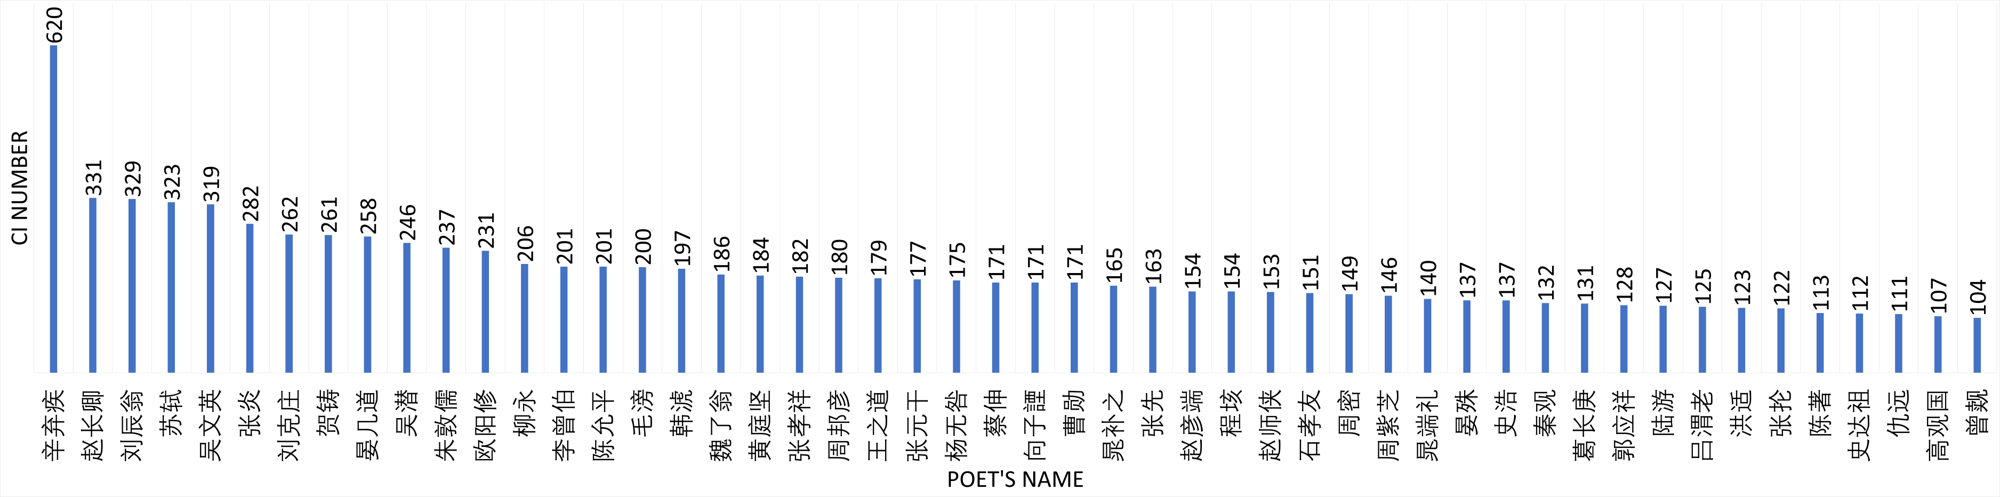
\includegraphics[width=0.9\linewidth]{poets.png}
%	\caption{Poem Number Created by Top 50 Productive Poets}
%	\label{fig:poet}
%\end{figure}

\begin{figure}[htbp]
	\centering
	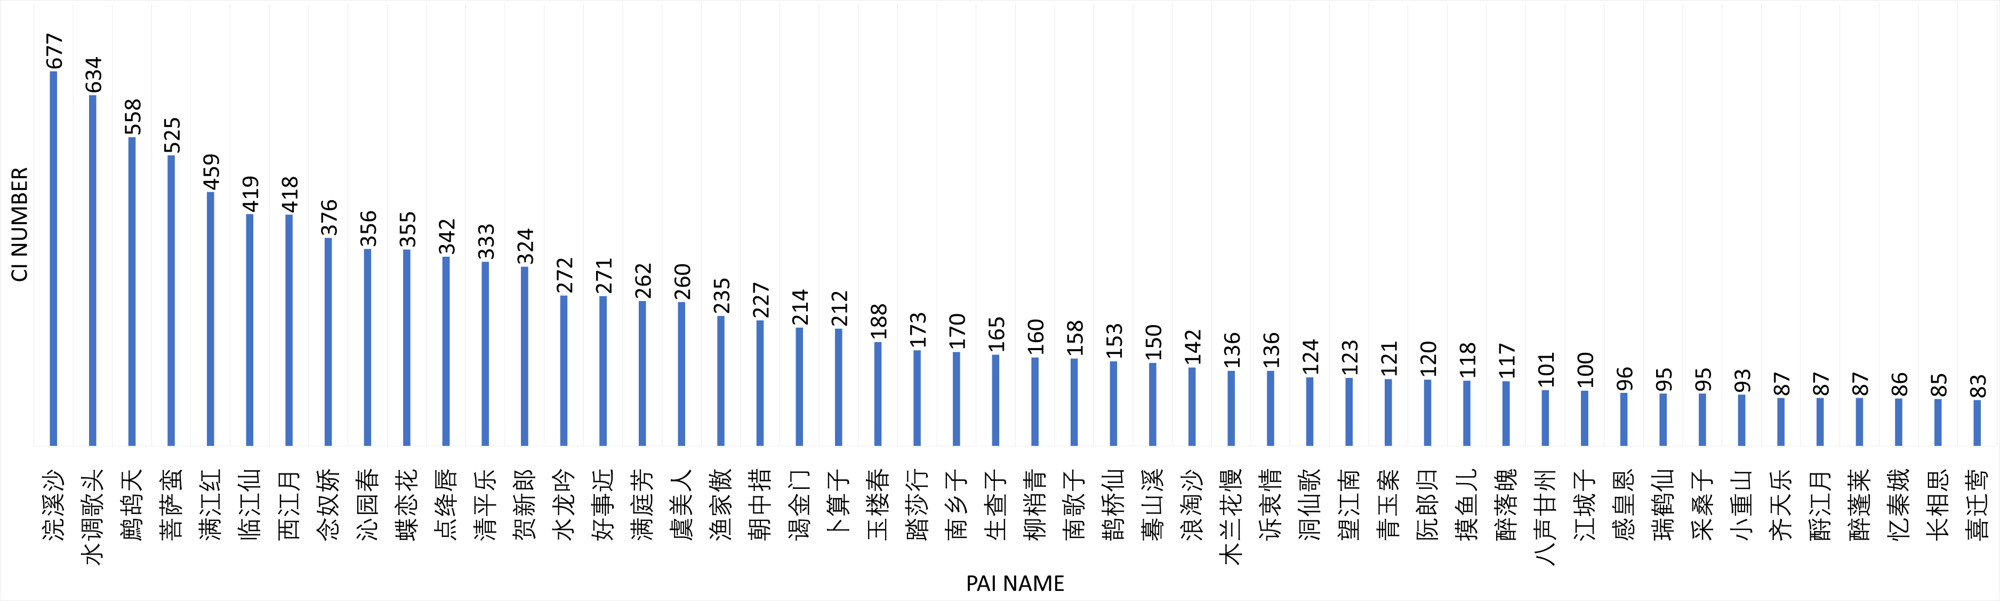
\includegraphics[width=0.9\linewidth]{Pai.png}
	\caption{Poem number of top 50 popular Pai}
	\label{fig:pai}
\end{figure}
%
\subsection {Word Frequency Analysis}
Word frequency analysis is to statistic and analyze the number of important words in the text, which is an important method of text mining.
%
 It is a traditional and useful content analysis method. The basic principle is to determine the overall style and theme of the entire article by the frequency of the words. By analyzing the word frequency in the poems, we have a general understanding of the style of poems and the process of writing those the poem, which can help us get more familiar with the grammar rules and themes of Ci. The most commonly used words can reveal common theme of Ci and the corresponding feelings. For example, we analyzed word frequency of season in our database. The result is shown in Figure \ref{fig:season}. We found that spring related words reached 2606, these words appeared in our dataset for 9210 times. Followed by autumn, there are 1167 words associated with autumn and appeared 3992 times. The unique scene in spring and autumn can trigger people's emotions, which might be the reason that so many poems are related with these two seasons.
\begin{figure}[htbp]
	\centering
	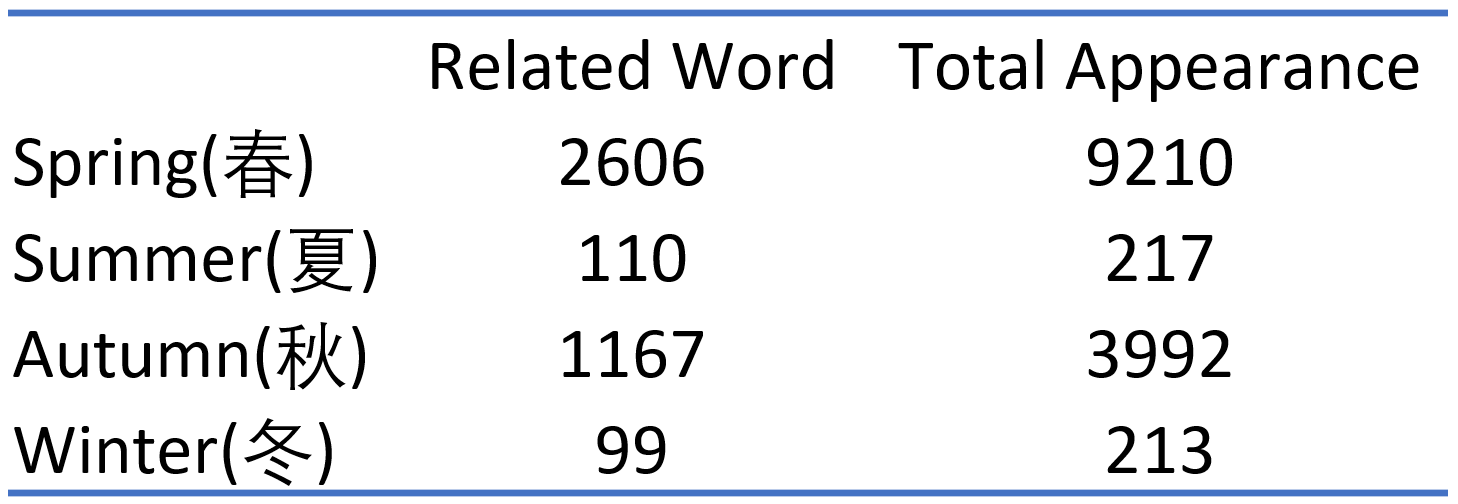
\includegraphics[width=0.8\linewidth]{season.png}
	\caption{Statistical data of season related word frequency in dataset}
	\label{fig:season}
\end{figure}
%
From most frequently used words, shown in Figure \ref{fig:wordcloud}, we found that the moon, east wind, mortal world, wine, dream, rain, flowers , sunset, old friends are the most commonly used images. Commonly used places, including Jiangnan, West Lake, Changan, Fairy Isle, Yangzhou. Commonly used verbs including laugh , come back, go back, lovesickness, look back, meet by chance. Commonly used emotions are hate, worry, hard, sigh, desolate, haggard. These words represent a very broad theme and style of Ci, including the description of leaving and missing, pride and enthusiasm, seasonal terms, chanting things, chanting nostalgia and so on.
%
\begin{figure}[htbp]
	\centering
	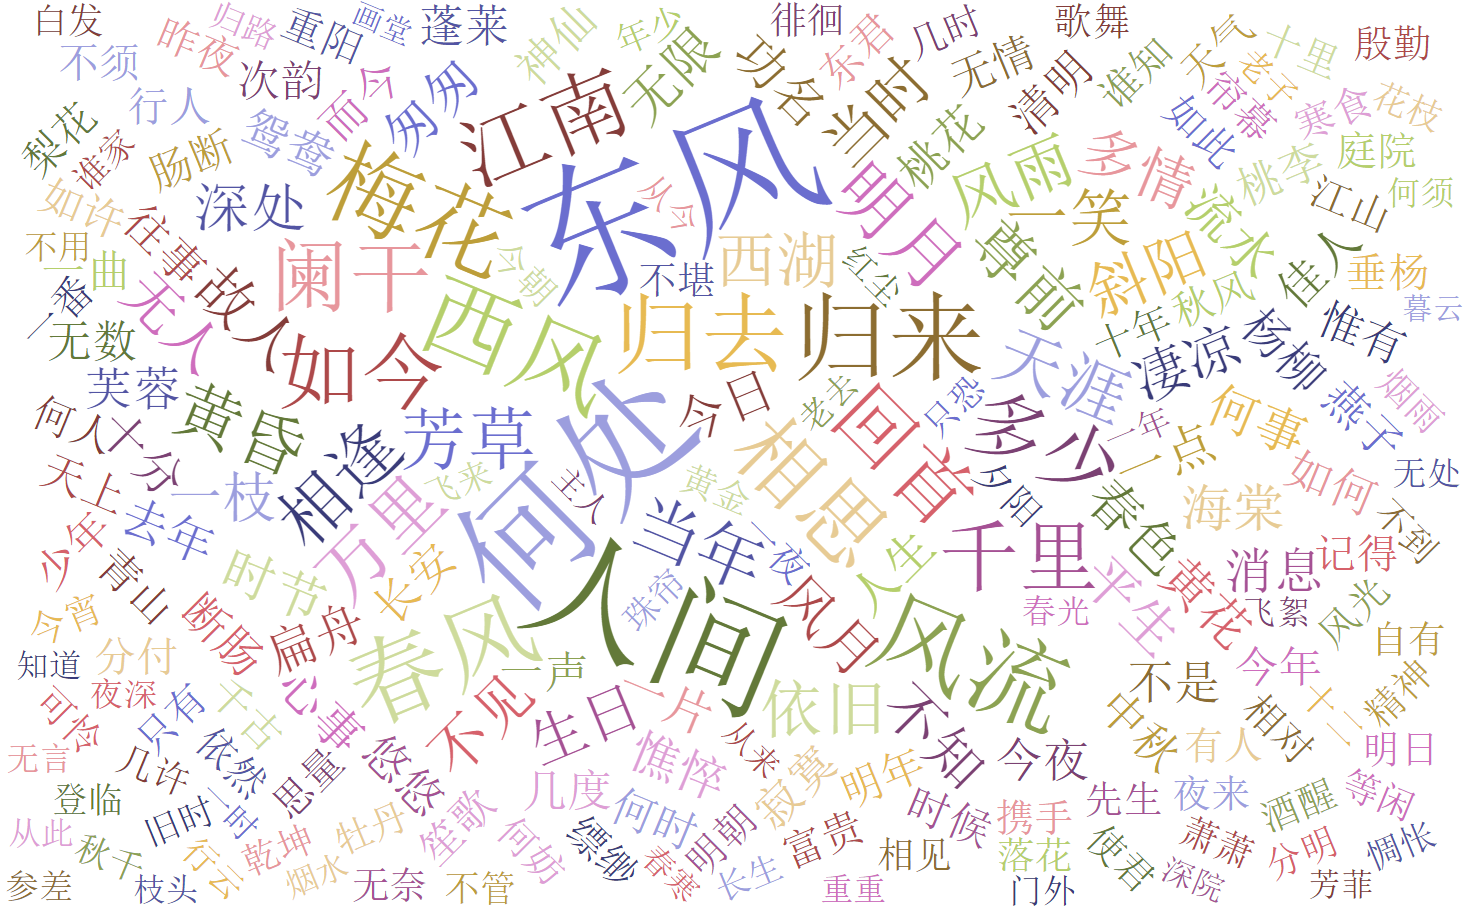
\includegraphics[width=0.8\linewidth] {wordcloud}
	\caption{Word could of frequently used words in dataset}
	\label{fig:wordcloud}
\end{figure}